\documentclass[11pt,]{article}
\usepackage{lmodern}
\usepackage{amssymb,amsmath}
\usepackage{ifxetex,ifluatex}
\usepackage{fixltx2e} % provides \textsubscript
\ifnum 0\ifxetex 1\fi\ifluatex 1\fi=0 % if pdftex
  \usepackage[T1]{fontenc}
  \usepackage[utf8]{inputenc}
\else % if luatex or xelatex
  \ifxetex
    \usepackage{mathspec}
    \usepackage{xltxtra,xunicode}
  \else
    \usepackage{fontspec}
  \fi
  \defaultfontfeatures{Mapping=tex-text,Scale=MatchLowercase}
  \newcommand{\euro}{€}
\fi
% use upquote if available, for straight quotes in verbatim environments
\IfFileExists{upquote.sty}{\usepackage{upquote}}{}
% use microtype if available
\IfFileExists{microtype.sty}{%
\usepackage{microtype}
\UseMicrotypeSet[protrusion]{basicmath} % disable protrusion for tt fonts
}{}
\usepackage[margin=1in]{geometry}
\usepackage{graphicx}
\makeatletter
\def\maxwidth{\ifdim\Gin@nat@width>\linewidth\linewidth\else\Gin@nat@width\fi}
\def\maxheight{\ifdim\Gin@nat@height>\textheight\textheight\else\Gin@nat@height\fi}
\makeatother
% Scale images if necessary, so that they will not overflow the page
% margins by default, and it is still possible to overwrite the defaults
% using explicit options in \includegraphics[width, height, ...]{}
\setkeys{Gin}{width=\maxwidth,height=\maxheight,keepaspectratio}
\ifxetex
  \usepackage[setpagesize=false, % page size defined by xetex
              unicode=false, % unicode breaks when used with xetex
              xetex]{hyperref}
\else
  \usepackage[unicode=true]{hyperref}
\fi
\hypersetup{breaklinks=true,
            bookmarks=true,
            pdfauthor={},
            pdftitle={},
            colorlinks=true,
            citecolor=blue,
            urlcolor=blue,
            linkcolor=magenta,
            pdfborder={0 0 0}}
\urlstyle{same}  % don't use monospace font for urls
\setlength{\parindent}{0pt}
\setlength{\parskip}{6pt plus 2pt minus 1pt}
\setlength{\emergencystretch}{3em}  % prevent overfull lines
\setcounter{secnumdepth}{0}

%%% Use protect on footnotes to avoid problems with footnotes in titles
\let\rmarkdownfootnote\footnote%
\def\footnote{\protect\rmarkdownfootnote}

%%% Change title format to be more compact
\usepackage{titling}

% Create subtitle command for use in maketitle
\newcommand{\subtitle}[1]{
  \posttitle{
    \begin{center}\large#1\end{center}
    }
}

\setlength{\droptitle}{-2em}
  \title{}
  \pretitle{\vspace{\droptitle}}
  \posttitle{}
  \author{}
  \preauthor{}\postauthor{}
  \date{}
  \predate{}\postdate{}

% load packages
\usepackage{amsmath,amsfonts,float,makecell,titletoc,titlesec,tocloft,titling,natbib,pdfpages,lineno,booktabs}
\usepackage[T1]{fontenc}
\usepackage{lmodern}
\usepackage[utf8]{inputenc}
\usepackage[doublespacing]{setspace}

% format captions
\usepackage[labelfont={small,bf}, labelsep=space, font={small}]{caption}

% format toc
%\renewcommand\cftsubsecfont{\normalfont\normalsize\bfseries}
% \renewcommand\cftsubsubsecfont{\normalfont\normalsize\bfseries}
% \renewcommand\cftparafont{\normalfont\normalsize\bfseries}
% \renewcommand\cftsubparafont{\normalfont\normalsize\itshape}

% line numbers
\linenumbers

% format abstract
\renewcommand{\abstractname}{Summary}
\renewenvironment{abstract}
 {\small
  \begin{center}
  \bfseries \abstractname\vspace{-.5em}\vspace{0pt}
  \end{center}
  \list{} {%
   \setlength{\leftmargin}{2mm}
   \setlength{\rightmargin}{\leftmargin}%
  }%
  \item\relax}
{\endlist}

% format section headers
\titleformat*{\section}{\Large\bfseries}
\titleformat{\subsection}[display]
	{\large\sffamily\lsstyle}
	{\subsectiontitlename\ \thesubsection}
	{0.5em}{}
\titleformat*{\subsubsection}{\large\itshape}

% make figures static
\let\origfigure\figure
\let\endorigfigure\endfigure
\renewenvironment{figure}[1][2] {
	\expandafter\origfigure\expandafter[H]
} {
	\endorigfigure
}

% define struts for tables
\newcommand\T{\rule{0pt}{2.6ex}} % top strut
\newcommand\B{\rule[-1.2ex]{0pt}{0pt}} % bottom strut

% define command to put new lines in table cells
%\newcommand{\specialcell}[2][c]{%
%  \begin{tabular}[#1]{@{}c@{}}#2\end{tabular}}
% insert S before figure and table caption
\pagenumbering{gobble}


\begin{document}

\maketitle


\subsection{Figures}\label{figures}

\begin{figure}[htbp]
\centering
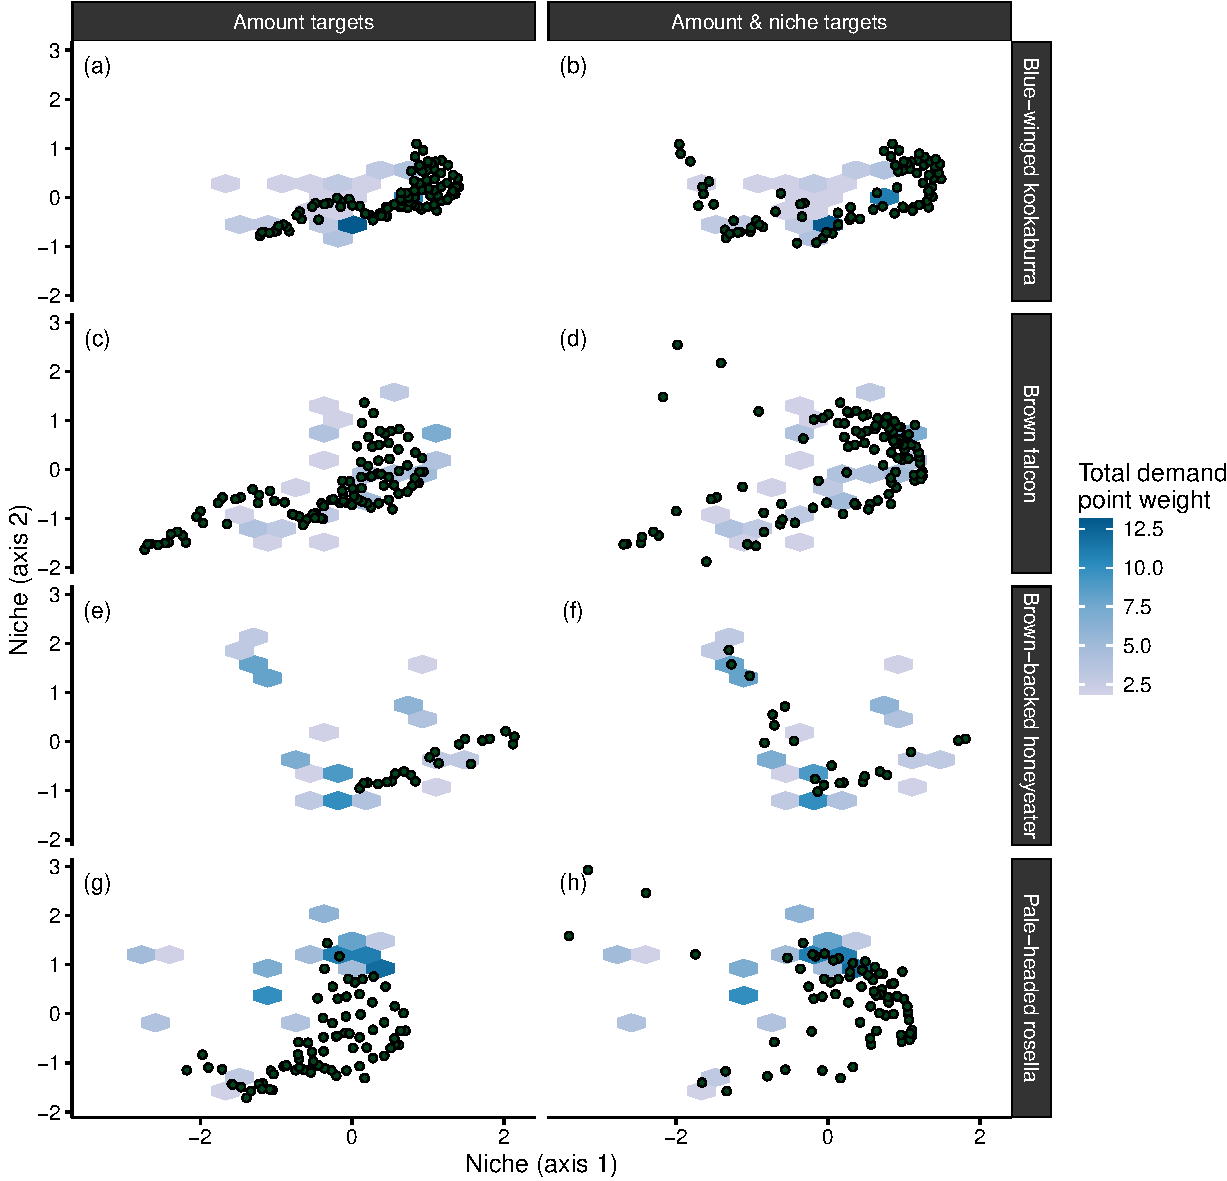
\includegraphics{figures_files/figure-latex/unnamed-chunk-3-1.pdf}
\caption{Example of an attribute space. This environmental attribute
space has dimensions relating to annual temperature ($^{\circ}$C) and
rainfall (mm) values. Letters denote the environmental conditions
associated with the geographic locations where four hypothetical
populations are found. Points represent demand points. In this space,
populations closer to each other are considered more similar to each
other.}
\end{figure}

\begin{figure}[htbp]
\centering
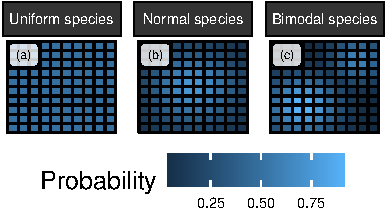
\includegraphics{figures_files/figure-latex/unnamed-chunk-4-1.pdf}
\caption{Simulated distributions of three species. Squares denote
planning units. The color of each planning unit indicates the
probability that each species inhabits it. Panel (a) shows the uniformly
distributed species, panel (b) shows the normally distributed species,
and panel (c) shows the bimodally distributed species.}
\end{figure}

\begin{figure}[htbp]
\centering
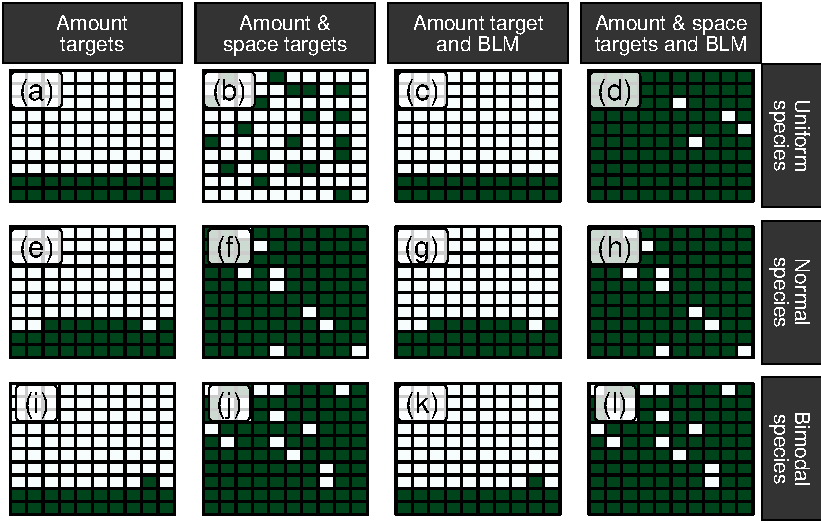
\includegraphics{figures_files/figure-latex/unnamed-chunk-5-1.pdf}
\caption{Simulation study prioritisations. Each panel shows a
prioritisation generated for a single species using a set of parameters.
Squares denote planning units, with dark green showing those planning
units selected for protection in a particular prioritisation. The top
row of panels (a, d, g, j) shows prioritisations generated for the
uniformly distributed species, middle row of panels (b, e, h, k) for the
normally distributed species, and the bottom row of panels (c, f, i, l)
for the bimodally distributed species. Each column of panels corresponds
to a different set of parameters used to generate the prioritisation.
The left column of panels (a--c) shows prioritizations generated using
only 20 \% amount targets, the middle-left column of panels (d--f) for
prioritisations generated using 20 \% amount and 75 \% space targets,
the middle-right column of panels (g--i) for prioritisations generated
using 20 \% amount based targets and a boundary length modifier (BLM) of
1, and the right column of panels (j--l) for prioritisations generated
using 20 \% amount and 75 \% space targets and also a boundary length
modifier of 1.}
\end{figure}

\begin{figure}[htbp]
\centering
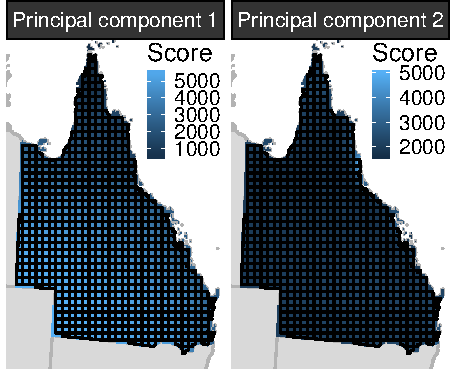
\includegraphics{figures_files/figure-latex/unnamed-chunk-6-1.pdf}
\caption{Distribution of environmental variation across Queensland,
Australia. Squares denote planning units. The panels show the first and
second main gradients of climatic variation.}
\end{figure}

\begin{figure}[htbp]
\centering
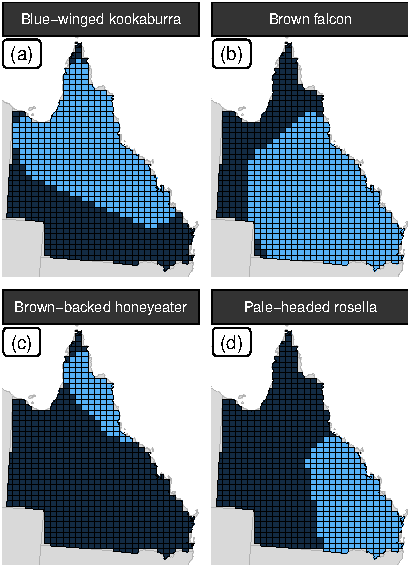
\includegraphics{figures_files/figure-latex/unnamed-chunk-7-1.pdf}
\caption{Distribution of the species used in the first case-study.
Squares denote planning units. Each panel shows the distribution of a
different species.}
\end{figure}

\begin{figure}[htbp]
\centering
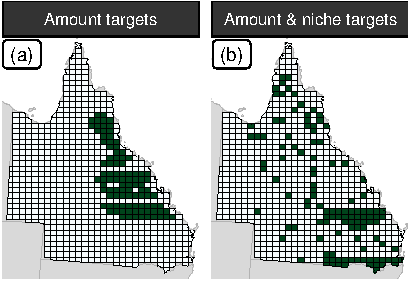
\includegraphics{figures_files/figure-latex/unnamed-chunk-8-1.pdf}
\caption{Prioritisations for the niche-based case-study in Queensland,
Australia. Squares represent planning units. Dark green planning units
for selected for protection and pale green units were discarded. Panel
(a) shows the planning units selected when using 20 \% amount targets.
Panel (b) shows the planning units selected selected when using 20 \%
amount targets and 75 \% niche targets}
\end{figure}

\begin{figure}[htbp]
\centering
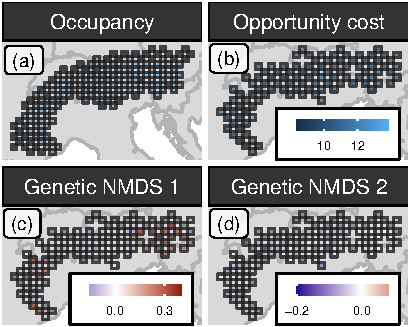
\includegraphics{figures_files/figure-latex/unnamed-chunk-9-1.pdf}
\caption{Study area and data used in the second case-study. Squares
denote planning units. Panel (a) shows all grid cells surveyed by the
IntraBioDiv project. Grid cells occupied by Betony-leaved Rampion are
shown in bright blue. The subsequent panels contain only the grid cells
that were occupied by the species. Panel (b) shows the opportunity cost
of each planning unit (estimated as the total human population density).
Panels (c--d) show the spatial distribution of the ordinated genetic
data. These values describe the typical genetic characteristics of
individuals in each planning unit. Planning units with similar
values/colors contain individuals with similar loci polymorphisms.}
\end{figure}

\begin{figure}[htbp]
\centering
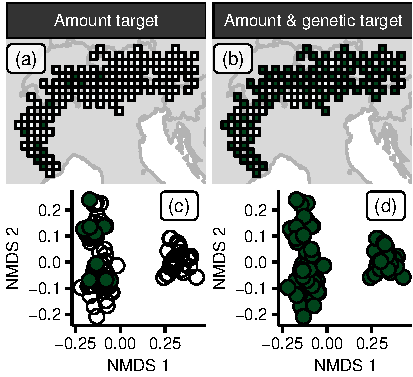
\includegraphics{figures_files/figure-latex/unnamed-chunk-10-1.pdf}
\caption{Prioritisations for the genetic case-study in the European
Alps. Panels (a--b) show prioritisations generated using different
parameters. Squares denote planning units shown in geographic space.
Panel (a) shows the planning units selected when using 10 \% amount
targets. Panel (b) shows the planning units selected when using 10 \%
amount targets and 95 \% genetic targets. Panels (c--d) show the
solutions in the genetic space. Each point corresponds to a planning
unit. The coordinates of the points represent the typical genetic
characeristics of individuals sampled in that planning unit (based on an
NMDS of the binary loci data). Planning units associated with points
that are closer togeather contain individuals with more similar genetic
characteristics than planning units that are further apart. In all
panels, dark green planning units were selected for protection, and pale
green planning units were discarded.}
\end{figure}

\end{document}
